
\begin{myex}
	
	\textbf{Hauteur des arbres dans une pépinière}
	
	\begin{multicols*}{2}
	
		\begin{center}
			\begin{tabular}{|@{\ }c@{\ }|@{\ }c@{\ }|}
				\hline
				Hauteur (en cm) & Nombre d'arbres \\ \hline
				$\intervFO{0}{100}$ & 20  \\ \hline
				$\intervFO{100}{200}$ & 12 \\ \hline
				$\intervFO{200}{300}$ & 49 \\ \hline
			\end{tabular}
		\end{center}
		
		
		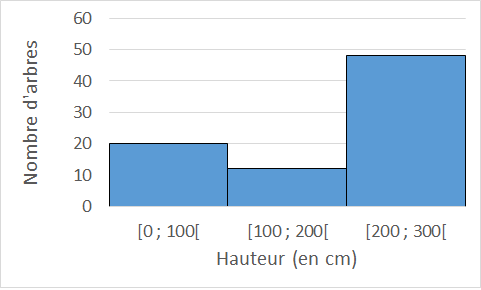
\includegraphics[scale=0.8]{img/histo}
	\end{multicols*}
	
\end{myex}

